Every chapter so far assumes access to a scalar reward signal: dynamic programming requires $r(s,a)$, model-free RL observes $r_t$ after each transition, and the Bellman optimality equation presupposes that rewards are known or observable. When they are neither, the DP/RL machinery cannot be applied directly.

In many domains, scalar rewards are unavailable but ordinal preferences over trajectories are easy to elicit. A human evaluator cannot assign a meaningful numerical score to a paragraph of text, but can reliably say ``response A is better than response B.'' The raw data is a set of trajectory pairs with binary preference labels. RLHF uses these ordinal comparisons to learn a proxy reward function $r_\theta$, which then serves as the scalar signal for standard RL optimization. This is not an inverse problem in the IRL sense; the goal is not to rationalize observed behavior, but rather a two-stage forward problem in which the analyst first learns a reward from human judgments and then solves the resulting MDP. \citet{christiano:2017} demonstrated that this approach could train agents without an explicit reward function. RLHF has since become the predominant method for aligning large language models.

\subsection{Learning Rewards from Preferences}

The canonical RLHF framework is built on a formal model of human preference. The observed data consists of tuples $(s, y_w, y_l)$, where $s$ is a context, and $y_w$ and $y_l$ are two outputs, with $y_w$ being the ``winner'' preferred by a human. Assuming preferences follow a latent utility model, the Bradley-Terry model \citep{bradley1952rank} gives the probability that $y_w$ is preferred: $P(y_w \succ y_l | s) = \sigma(r_\theta(s, y_w) - r_\theta(s, y_l))$, where $r_\theta: \mathcal{S} \times \mathcal{Y} \to \mathbb{R}$ is a learned \textit{reward model} parameterized by $\theta$, trained to approximate human preferences (not the ground-truth reward, which is unobserved), and $\sigma(\cdot)$ is the logistic function. This formulation is a binary logit model (Section~\ref{section:language}, Equation~\ref{eq:softmax_logit}). The reward model parameters $\theta$ are estimated by minimizing the negative log-likelihood of the observed human choices:
\begin{equation}
    \mathcal{L}(\theta) = -\mathbb{E}_{(s, y_w, y_l) \sim \mathcal{D}} \left[ \log \sigma \left( r_\theta(s, y_w) - r_\theta(s, y_l) \right) \right],
\label{eq:rlhf_loss}
\end{equation}
In the LLM setting, the ``outputs'' $y_w$ and $y_l$ are token sequences, i.e., trajectories of the autoregressive policy, so preferences are over trajectories rather than single actions. The preference loss in Equation~(\ref{eq:rlhf_loss}) is MLE of a choice model where the ``alternatives'' are trajectory segments and the ``choice'' is the human-preferred one.

\subsection{The RLHF Pipeline and Direct Optimization}

The learned $r_\theta$ then serves as a proxy objective for policy optimization. Building on the reward-learning and RL fine-tuning framework of \citet{ziegler2019fine} and \citet{stiennon2020learning}, the canonical three-stage pipeline was formalized by \citet{ouyang2022training}. First, a base pretrained model is initialized via supervised fine-tuning (SFT) on a small dataset of high-quality demonstrations, yielding an initial policy $\pi^{SFT}$. This grounds the model in the desired style and format. The second step is the reward model training as described, using preference data generated from this $\pi^{SFT}$.

In the third step, the SFT policy $\pi_\phi$ is fine-tuned via PPO (Section~\ref{sec:actor_critic}) to maximize the frozen reward model $r_\theta$, with a KL-divergence penalty preventing the policy from drifting into regions where $r_\theta$ is unreliable. The objective is
\begin{equation}
    J(\phi) = \mathbb{E}_{s \sim \mathcal{D}, y \sim \pi_\phi(\cdot|s)} [r_\theta(s, y)] - \lambda_{KL} \mathbb{E}_{s \sim \mathcal{D}} [D_{KL}(\pi_\phi(\cdot|s) \,||\, \pi^{SFT}(\cdot|s))],
\label{eq:rlhf_objective}
\end{equation}
where $D_{KL}$ is the Kullback-Leibler divergence and $\lambda_{KL}$ controls the penalty strength.\footnote{$\lambda_{KL}$ denotes the KL penalty weight, reserving $\beta$ for model parameters and $\gamma$ for discount factors. The standard RLHF literature, including \citet{rafailov2023direct}, uses $\beta$ for this parameter.} Without this constraint, the policy exploits inaccuracies in $r_\theta$ to achieve high proxy scores with degenerate behavior (``reward hacking''), the RLHF analogue of divergence under function approximation (Section~\ref{sec:deadly_triad}).

The KL-regularized objective in Equation~(\ref{eq:rlhf_objective}) admits a Bayesian interpretation \citep{korbak2022rl}. In this view, the reference policy $\pi^{SFT}$ acts as a prior distribution over plausible responses. The reward model $r_\theta$ provides evidence, specifying which responses are more desirable. The goal of alignment is to find the posterior distribution $\pi^*$ that optimally combines the prior with this evidence. This ideal posterior policy takes the form of Equation~(\ref{eq:rlhf_posterior}):
\begin{equation}
    \pi^*(y|s) \propto \pi^{SFT}(y|s) \exp\left(\frac{r_\theta(s, y)}{\lambda_{KL}}\right).
\label{eq:rlhf_posterior}
\end{equation}
The reward function scaled by $\lambda_{KL}$ defines the log-likelihood, so the KL-regularized objective $J(\phi)$ is equivalent (up to an additive constant) to the Evidence Lower Bound (ELBO) for this Bayesian inference problem. Maximizing the RLHF objective via PPO is therefore variational inference: finding the policy $\pi_\phi$ that minimizes KL divergence to $\pi^*$. This reframes the KL penalty as a structural component of the inference problem rather than an ad-hoc regularizer.

Despite this closed-form characterization, the three-stage RLHF pipeline is complex to implement, requiring training multiple large models and a computationally expensive RL loop. Direct Preference Optimization (DPO), introduced by \citet{rafailov2023direct}, collapses the pipeline into a single supervised learning objective by reparameterizing the reward function in terms of $\pi^*$ and $\pi^{SFT}$, as in Equation~(\ref{eq:dpo_reparameterize}):
\begin{equation}
    r(s,y) = \lambda_{KL} \log\left(\frac{\pi^*(y|s)}{\pi^{SFT}(y|s)}\right) + \lambda_{KL} \log Z(s).
\label{eq:dpo_reparameterize}
\end{equation}
When this analytical expression for the reward is substituted into the Bradley-Terry preference loss from Equation~(\ref{eq:rlhf_loss}), the unknown partition function $Z(s)$ cancels out. This yields a loss function that depends only on the policy $\pi_\phi$ being optimized and the fixed reference policy $\pi^{SFT}$. The DPO objective, given in Equation~(\ref{eq:dpo_loss}), is thus a simple binary cross-entropy loss over policy likelihoods:
\begin{equation}
    \mathcal{L}_{DPO}(\phi; \pi^{SFT}) = -\mathbb{E}_{(s, y_w, y_l) \sim \mathcal{D}} \left[ \log \sigma \left( \lambda_{KL} \log \frac{\pi_\phi(y_w|s)}{\pi^{SFT}(y_w|s)} - \lambda_{KL} \log \frac{\pi_\phi(y_l|s)}{\pi^{SFT}(y_l|s)} \right) \right].
\label{eq:dpo_loss}
\end{equation}
This objective is optimized on $\phi$ using standard supervised learning with a static preference dataset. The gradient increases the likelihood of preferred responses $y_w$ and decreases the likelihood of dispreferred responses $y_l$, relative to the reference policy.

\begin{figure}[t]
\centering
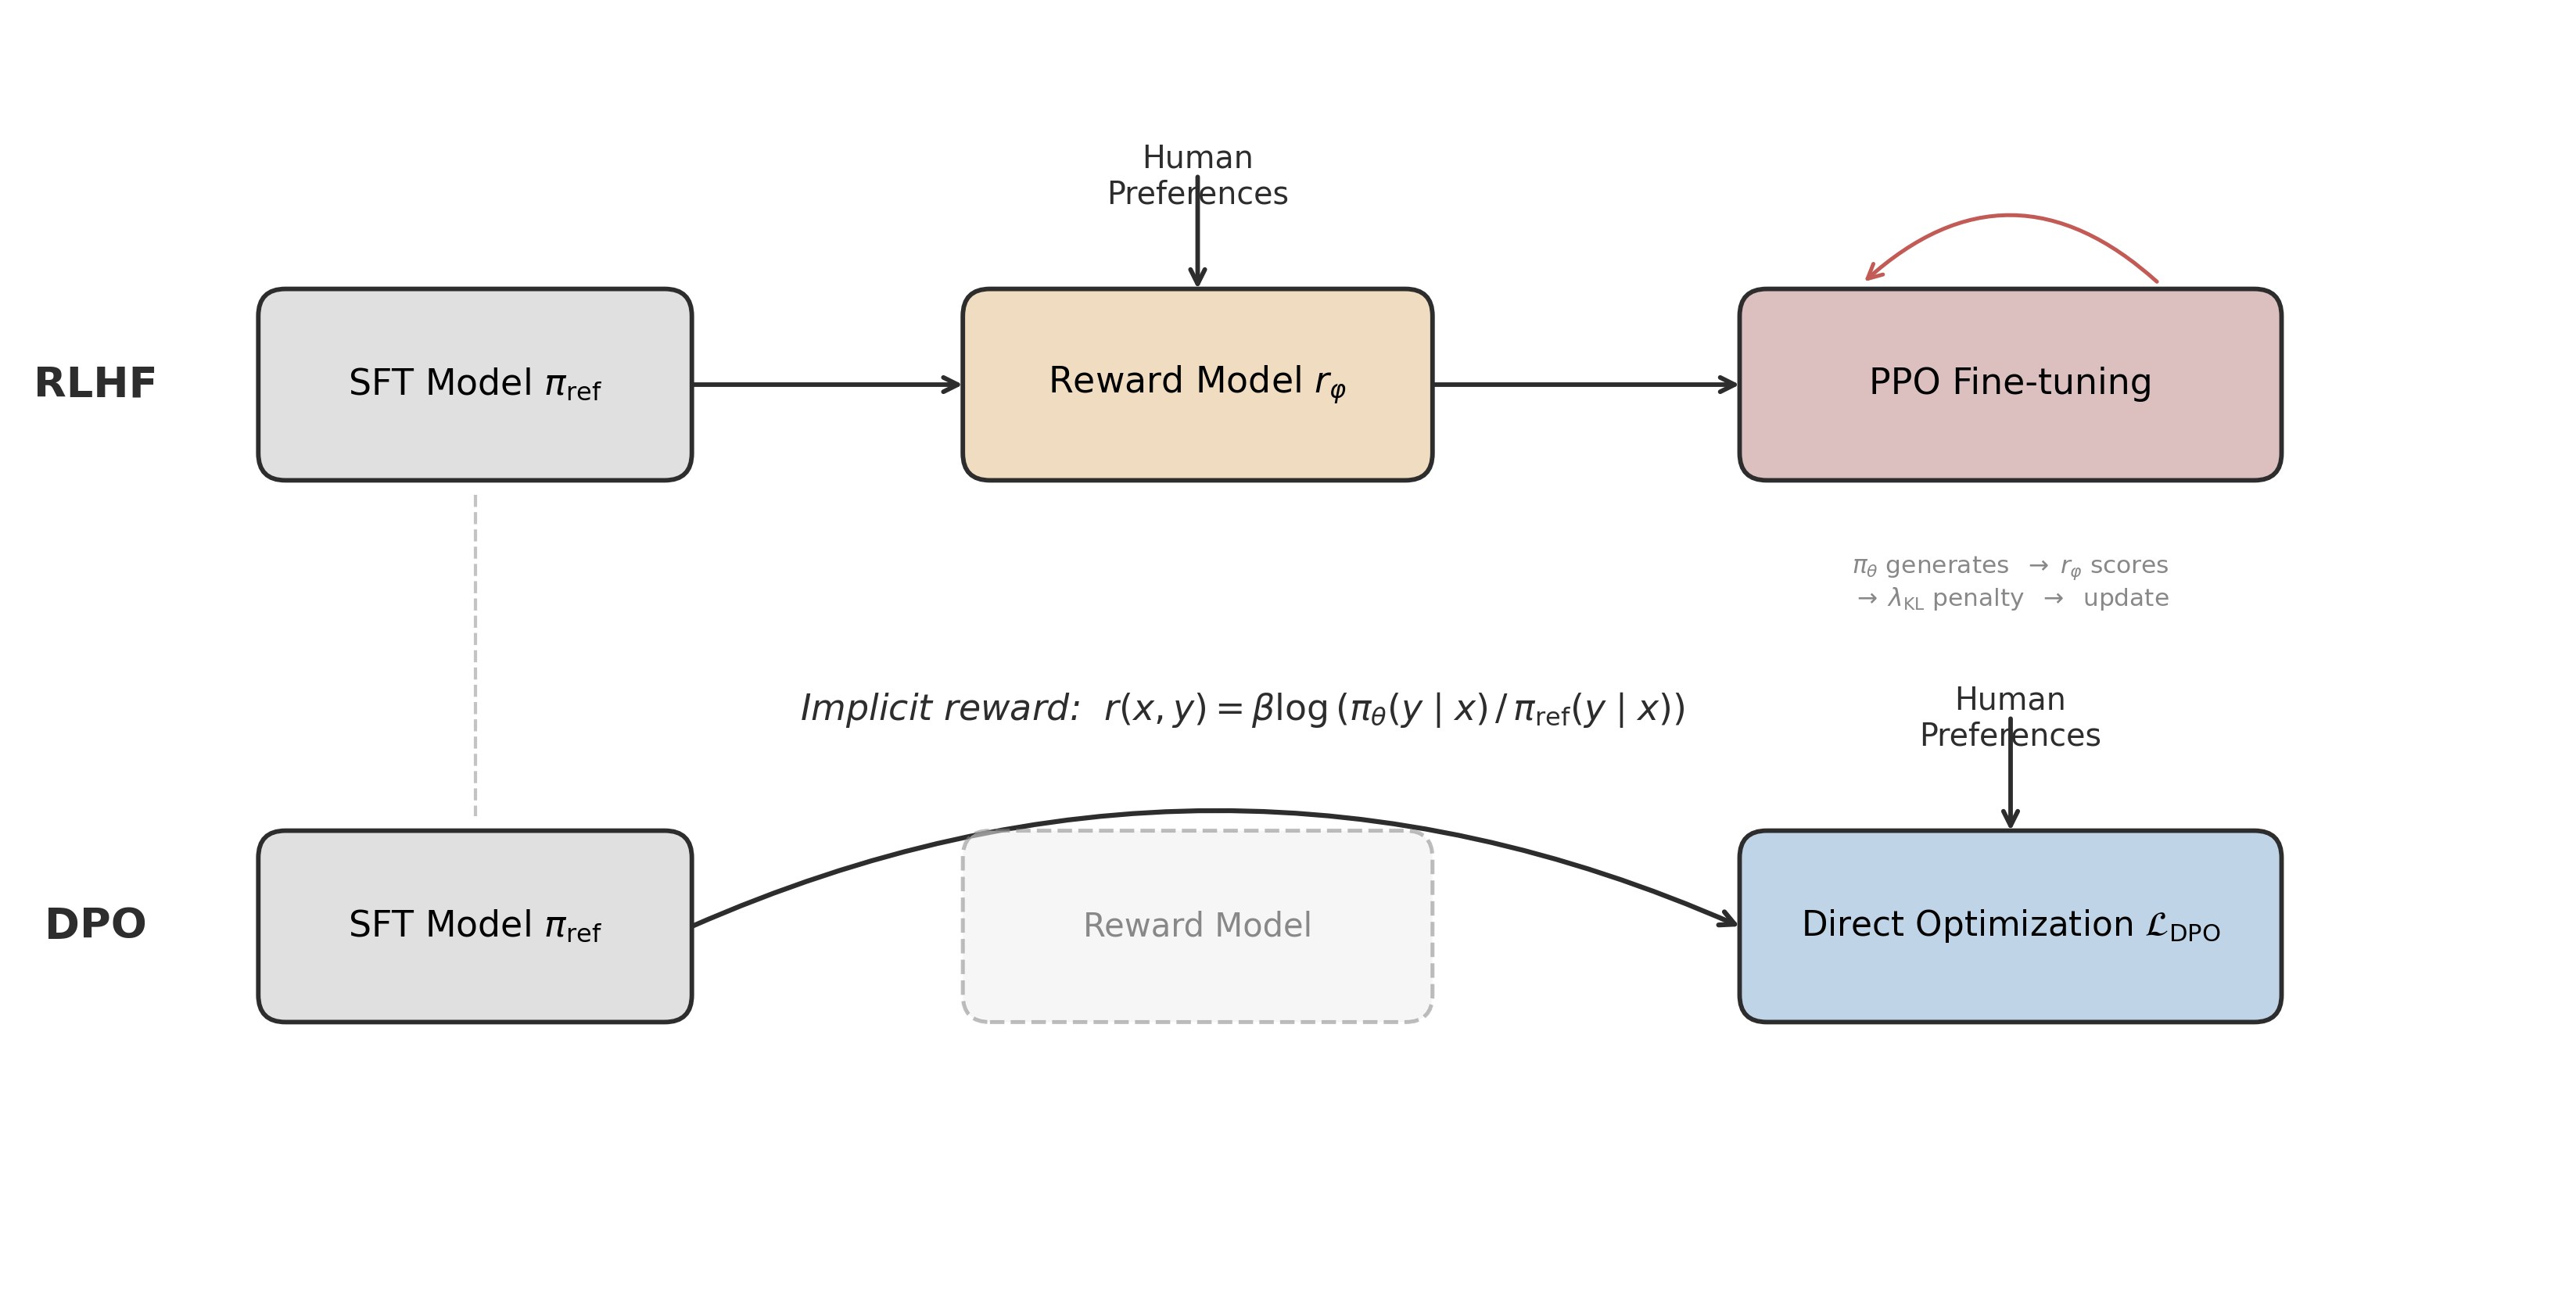
\includegraphics[width=\textwidth]{../ch08_rlhf/sims/rlhf_dpo_pipeline.png}
\caption{RLHF versus DPO pipelines. Top row: the three-stage RLHF pipeline trains a reward model from human preferences, then uses PPO to fine-tune the policy with a KL penalty. Bottom row: DPO collapses the pipeline into a single supervised learning objective over preference pairs, eliminating the explicit reward model (ghosted box).}
\label{fig:rlhf_dpo_pipeline}
\end{figure}

\subsection{Recent Developments}

A subsequent innovation leverages DPO to create an iterative self-improvement loop, reducing reliance on static, human-annotated data \citep{yuan2024self}. In this paradigm, dubbed Self-Rewarding Language Models, a single language model acts as both the instruction-following agent and its own reward model. The process begins with a base model fine-tuned to have both instruction-following and evaluation capabilities (``LLM-as-a-Judge''). In each subsequent iteration, the current model generates a new preference dataset for itself by producing multiple responses to a set of prompts and then evaluating its own outputs to assign scores. These scores are used to construct preference pairs $(y_w, y_l)$, which form an AI-generated feedback dataset. The model is then fine-tuned on this new data using the DPO loss. This iterative process creates a feedback loop where enhancements in instruction-following ability lead to better reward modeling, which in turn fuels the next round of policy optimization.

While RLHF and its successors have proven effective at aligning model behavior with human preferences, several open issues remain. The framework does not aim to solve the identification problem in the strict econometric sense; the learned reward model $r_\theta$ (whether explicit or implicit in DPO) is a proxy for preference, not necessarily the uniquely identified ``true'' utility function required for welfare analysis.\footnote{The identification problem in preference learning mirrors that in discrete choice. The reward function is identified only up to an additive constant and requires a location normalization.} Furthermore, the notion of ``human feedback'' is a significant simplification, as the preferences being optimized are those of a small, non-representative group of paid labelers, raising important questions about whose values are being embedded in these systems. Finally, the fine-tuning process can lead to degraded performance on standard academic benchmarks, a phenomenon called the \textit{alignment tax} \citep{ouyang2022training}.\footnote{The alignment tax, as described by \citet{ouyang2022training}, refers to performance regressions on public NLP benchmarks (SQuAD, DROP, HellaSwag) that result from RLHF fine-tuning.} Mitigating these challenges while scaling alignment beyond the limits of human data collection remains a key frontier for the field.

\subsection{Simulation Study: Preference Learning in Job Search}

A worker searches for jobs in a labor market with compensating differentials, following a McCall (1970)-style search model. Each job is characterized by a wage $w \in \{20, 28, 38, 50, 65, 82, 100, 125\}$ (thousands) and an amenity level $z \in \{0, 1, \ldots, 6\}$ capturing commute quality, flexibility, and job security. The state space has 112 states: 56 searching states in which the worker observes a pending offer $(w_i, z_j)$ and decides to accept or reject, plus 56 employed states $(w_i, z_j)$ in which the worker decides to stay or quit. The offer distribution exhibits compensating differentials, with wage rank and amenity rank negatively correlated ($\rho = -0.74$): high-wage offers cluster with low amenities and vice versa. The worker's true per-period utility is $u(w, z) = \alpha \log(w) + (1 - \alpha) z$ with $\alpha = 0.6$, but this function is unobserved; the worker can only compare career trajectories (``I prefer path A to path B''), exactly as in stated-preference surveys in labor economics. While searching, the worker receives the unemployment benefit $u_b = \alpha \log(b)$ where $b = 28$. Layoffs occur with probability $p = 0.05$ per period, and the discount factor is $\gamma = 0.95$. Dynamic programming gives $V^*(s_0) = 74.13$; the optimal policy accepts 25 of 56 offer types and stays employed at 25 of 56 job types. Preference data is generated by rolling out a uniform random policy from a random searching state. Each rollout produces a career segment of $L = 15$ periods recording states and actions. For each of $K$ comparisons, two independent career segments are generated; the segment with higher cumulative discounted utility under the true (unobserved) utility function is labeled as preferred via the Bradley-Terry model. Figure~\ref{fig:search_env} shows the optimal accept/reject and stay/quit boundaries.

\begin{figure}[htbp]
\centering
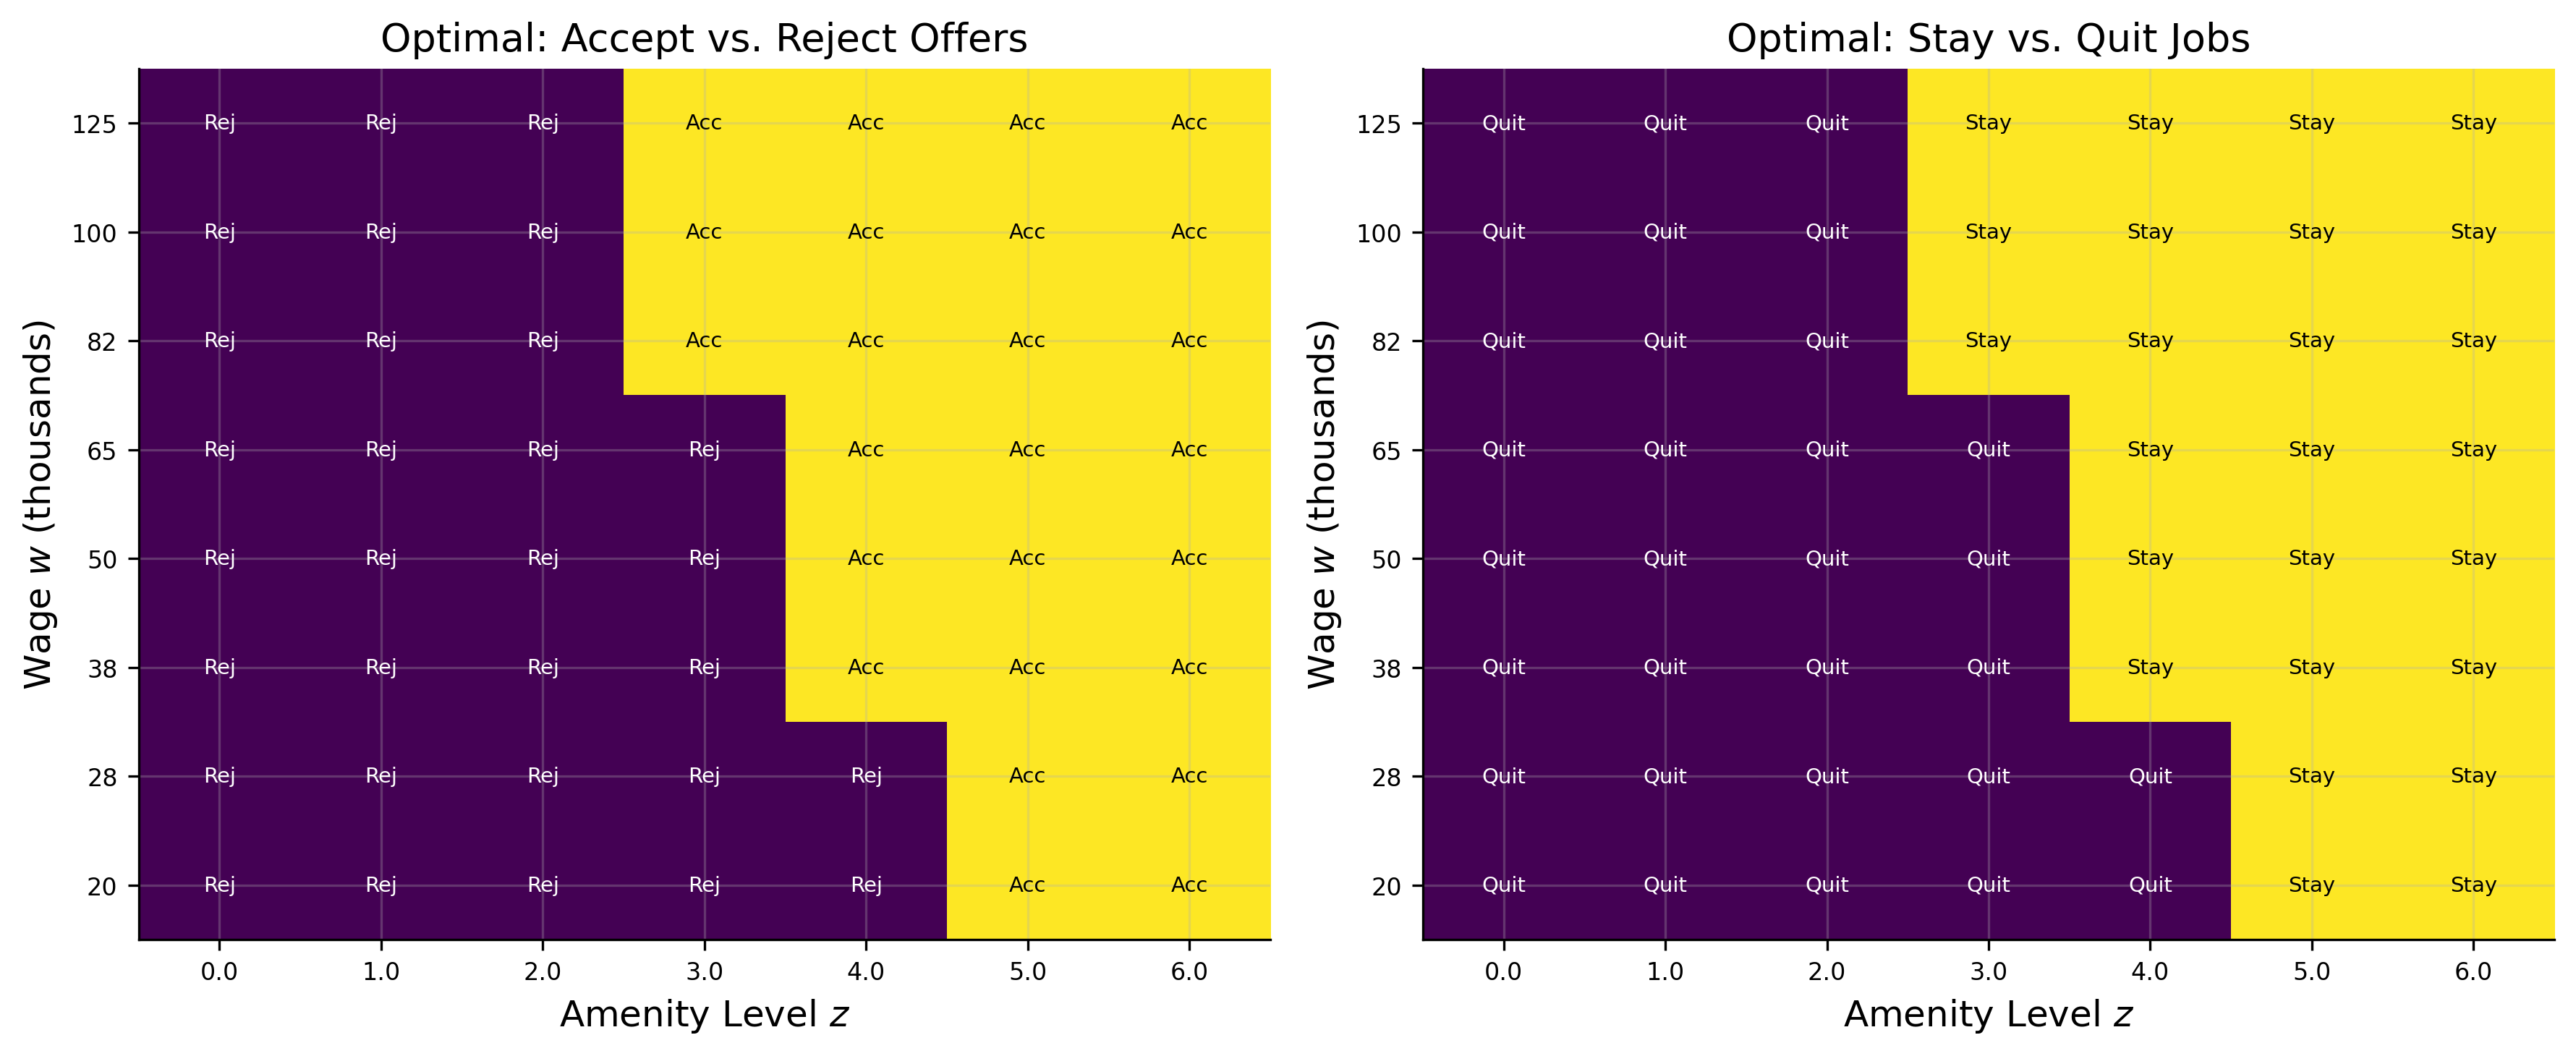
\includegraphics[width=0.85\textwidth]{../ch08_rlhf/sims/job_search_env.png}
\caption{Left: the optimal accept/reject boundary for searching states in wage-amenity space. Right: the optimal stay/quit boundary for employed states. Both boundaries cut diagonally, reflecting the tradeoff between wage and amenity quality under compensating differentials.}
\label{fig:search_env}
\end{figure}

Six methods are compared across $K \in \{25, 50, 100, 200, 500, 1{,}000, 2{,}000, 5{,}000\}$, averaged over 30 seeds. The neural network RLHF reward model is a two-layer MLP trained by Bradley-Terry MLE on the $K$ segment pairs; per-transition rewards are discount-weighted and summed to obtain a segment score, and the resulting 112-state reward table is solved by value iteration.\footnote{The neural network has 4 inputs (normalized log-wage, normalized amenity, employment indicator, action), 32 hidden units per layer, and $\sim$1{,}200 parameters. The logistic loss from Equation~(\ref{eq:rlhf_loss}) is applied to discount-weighted segment reward sums.} The correctly specified structural model parameterizes utility as $\hat{u} = \hat{\alpha} \log(w) + (1 - \hat{\alpha}) z$, estimating the single parameter $\hat{\alpha}$ via Bradley-Terry MLE, then solves the MDP. The misspecified model uses $\hat{u} = \hat{\alpha} \log(w) + (1 - \hat{\alpha}) \bar{z}$, where $\bar{z} = 3$ is the mean amenity level; this model ignores amenity variation across jobs, treating all amenities as identical. DPO trains a tabular softmax policy directly from trajectory comparisons, bypassing reward modeling entirely.\footnote{DPO uses 112 logit parameters $\phi_s$, one per state, trained via the DPO loss (Equation~\ref{eq:dpo_loss}) with Adam optimization over a sweep of $\lambda_{KL} \in \{0.01, 0.05, 0.1, 0.5, 1.0, 5.0\}$, selecting the $\lambda_{KL}$ that minimizes training loss. The reference policy is uniform: $\pi^{SFT}(a|s) = 0.5$. To match the LLM setup where both completions condition on the same prompt, DPO comparison pairs start from the same initial state.} Tabular Q-learning ($10{,}000$ episodes, $\varepsilon = 0.15$, learning rate $0.1$) and exact DP provide scalar-reward baselines. All four preference methods receive identical comparison data per seed; DPO receives a same-state variant generated from the same seed.

\begin{table}[htbp]
\centering
\caption{Sample complexity of preference-based policy learning on a McCall-style job search MDP with compensating differentials (30 seeds, $L = 15$). Six methods spanning four preference-learning approaches (structural, neural network, DPO) and two scalar-reward baselines (DP, Q-learning).}
\label{tab:preference_search}
\begin{tabular}{llrr}
\hline
Method & $K$ & $V^\pi(s_0)$ & \% of DP \\
\hline
DP Oracle & --- & $74.13$ & $100.0$ \\
Q-Learning & --- & $73.60 \pm 0.05$ & $99.3$ \\
\hline
NN RLHF & $25$ & $73.05 \pm 0.13$ & $98.5$ \\
DPO & $25$ & $66.39 \pm 0.34$ & $89.6$ \\
Correct & $25$ & $74.03 \pm 0.03$ & $99.9$ \\
Misspecified & $25$ & $67.34 \pm 0.38$ & $90.8$ \\
\hline
NN RLHF & $50$ & $73.31 \pm 0.08$ & $98.9$ \\
DPO & $50$ & $68.02 \pm 0.23$ & $91.8$ \\
Correct & $50$ & $74.07 \pm 0.02$ & $99.9$ \\
Misspecified & $50$ & $67.12 \pm 0.33$ & $90.6$ \\
\hline
NN RLHF & $100$ & $73.60 \pm 0.06$ & $99.3$ \\
DPO & $100$ & $69.25 \pm 0.18$ & $93.4$ \\
Correct & $100$ & $74.10 \pm 0.01$ & $100.0$ \\
Misspecified & $100$ & $67.24 \pm 0.28$ & $90.7$ \\
\hline
NN RLHF & $200$ & $73.85 \pm 0.05$ & $99.6$ \\
DPO & $200$ & $70.16 \pm 0.16$ & $94.6$ \\
Correct & $200$ & $74.12 \pm 0.00$ & $100.0$ \\
Misspecified & $200$ & $67.54 \pm 0.17$ & $91.1$ \\
\hline
NN RLHF & $500$ & $73.99 \pm 0.02$ & $99.8$ \\
DPO & $500$ & $70.60 \pm 0.10$ & $95.2$ \\
Correct & $500$ & $74.13 \pm 0.00$ & $100.0$ \\
Misspecified & $500$ & $67.55 \pm 0.15$ & $91.1$ \\
\hline
NN RLHF & $1000$ & $73.95 \pm 0.03$ & $99.8$ \\
DPO & $1000$ & $70.59 \pm 0.09$ & $95.2$ \\
Correct & $1000$ & $74.12 \pm 0.00$ & $100.0$ \\
Misspecified & $1000$ & $67.52 \pm 0.12$ & $91.1$ \\
\hline
NN RLHF & $2000$ & $74.04 \pm 0.02$ & $99.9$ \\
DPO & $2000$ & $70.41 \pm 0.07$ & $95.0$ \\
Correct & $2000$ & $74.13 \pm 0.00$ & $100.0$ \\
Misspecified & $2000$ & $67.41 \pm 0.11$ & $90.9$ \\
\hline
NN RLHF & $5000$ & $74.09 \pm 0.01$ & $99.9$ \\
DPO & $5000$ & $70.14 \pm 0.07$ & $94.6$ \\
Correct & $5000$ & $74.13 \pm 0.00$ & $100.0$ \\
Misspecified & $5000$ & $67.46 \pm 0.11$ & $91.0$ \\
\hline
\end{tabular}

\end{table}

\begin{figure}[htbp]
\centering
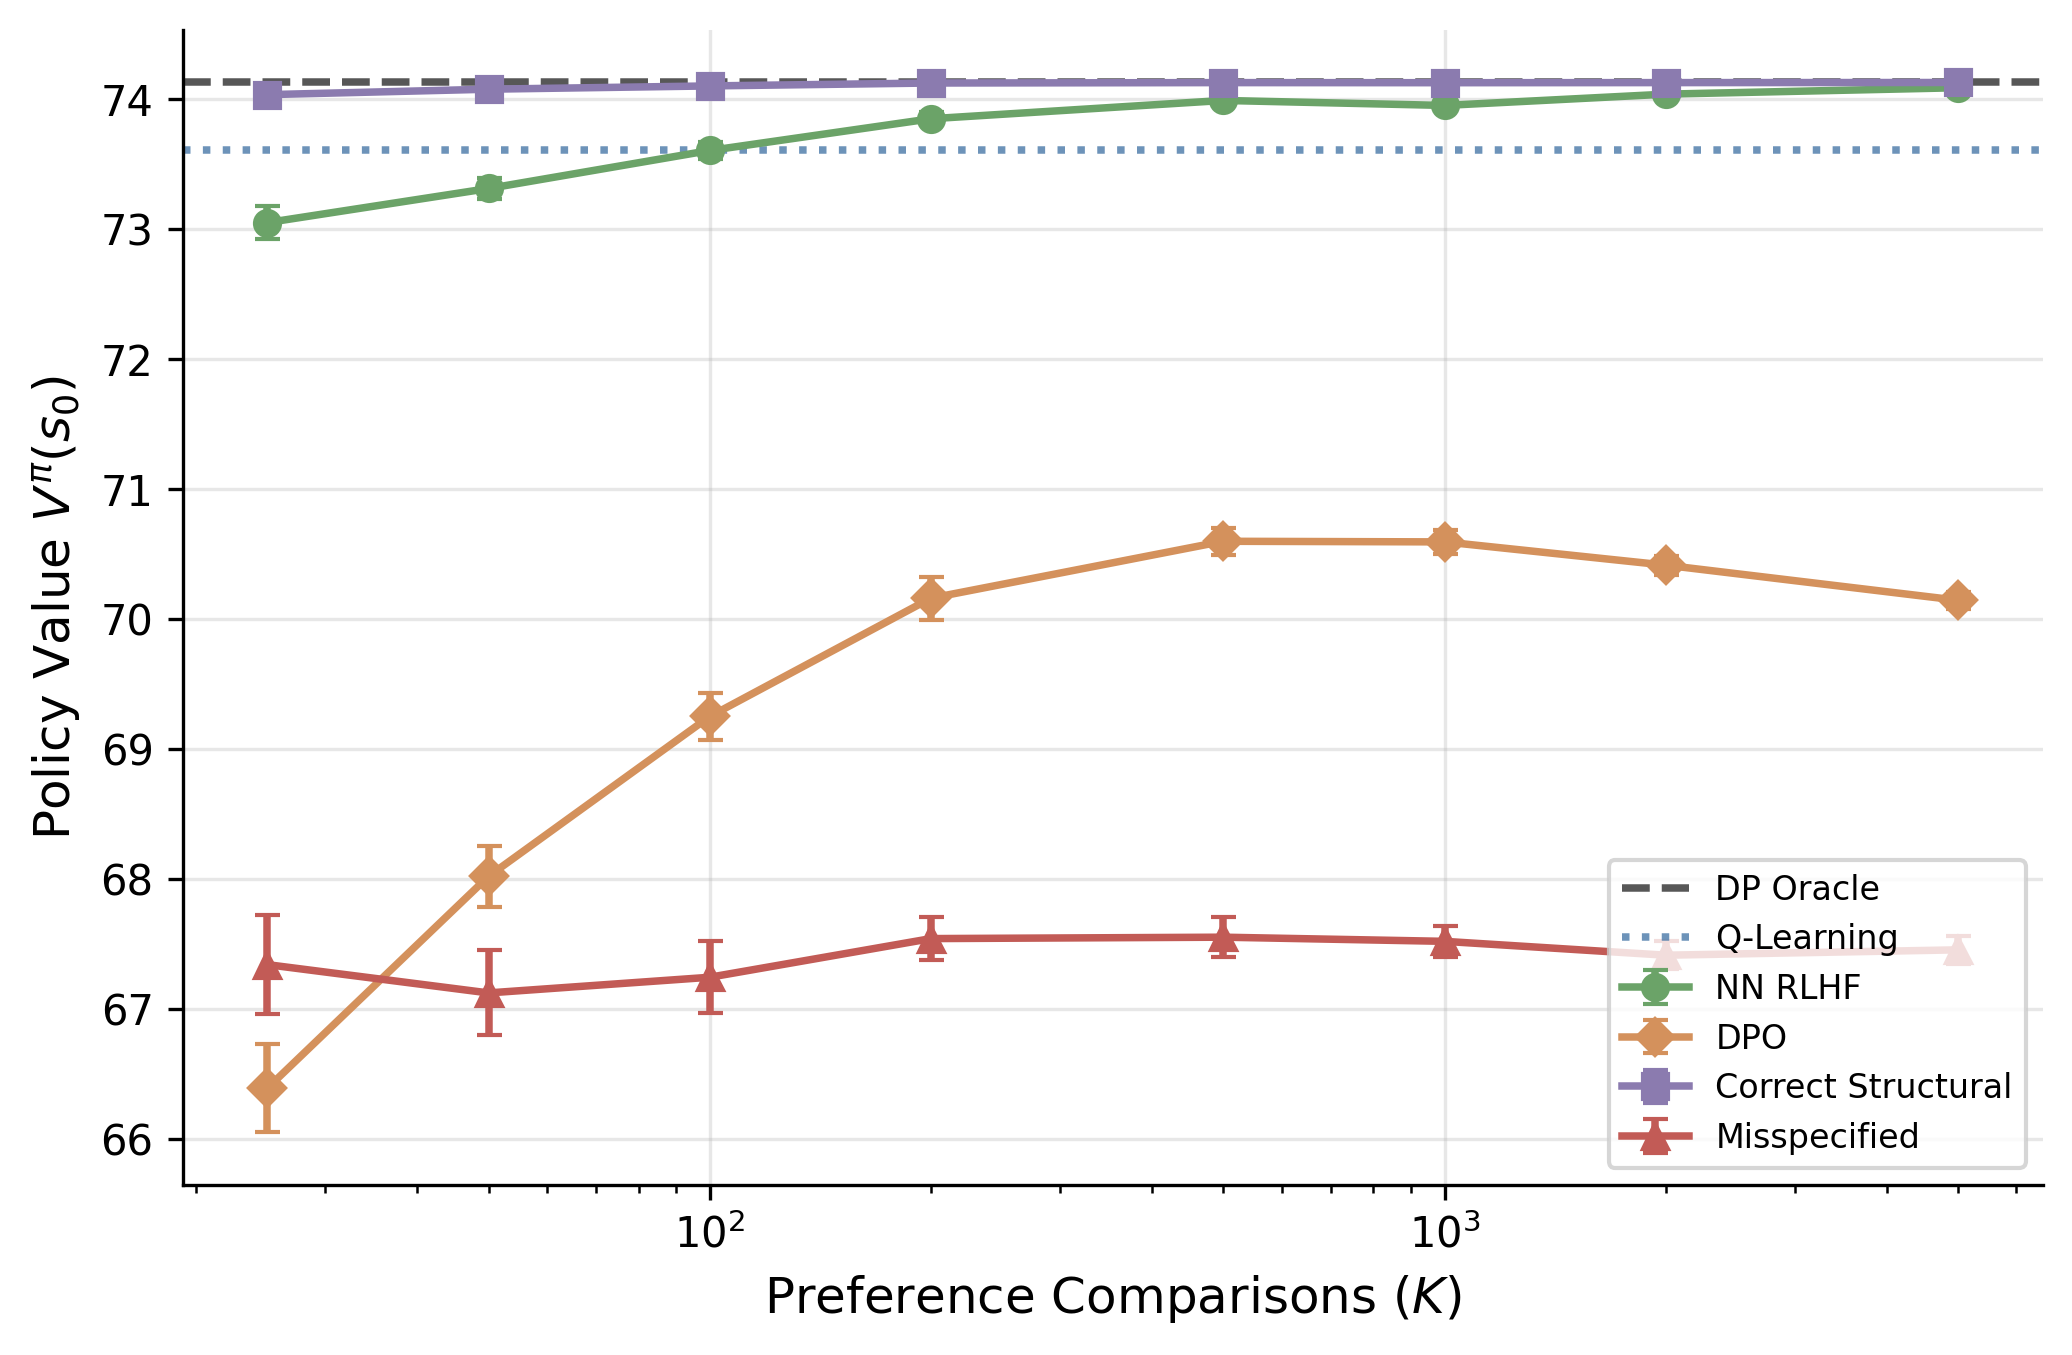
\includegraphics[width=0.7\textwidth]{../ch08_rlhf/sims/job_search_sample_complexity.png}
\caption{Policy value $V^\pi(s_0)$ versus number of preference comparisons $K$ for all six methods.}
\label{fig:preference_sample}
\end{figure}

Table~\ref{tab:preference_search} and Figure~\ref{fig:preference_sample} report the main results. Three findings stand out. First, the correctly specified structural model dominates: even at $K = 25$ it achieves 99.9\% of DP-optimal, illustrating the power of correct specification when the model has a single free parameter. Second, the neural network converges more slowly but reaches 99.9\% by $K = 5{,}000$, reflecting the higher sample complexity of a flexible model relative to a one-parameter structural specification. Third, DPO plateaus at approximately 95\% by $K = 500$ and does not improve further.\footnote{DPO learns only from $(s,a)$ pairs visited in training trajectories generated by the random behavioral policy. It cannot propagate value to undervisited states the way value iteration does after learning a reward model, so states poorly covered by the behavioral policy remain suboptimal regardless of $K$.} This plateau is qualitatively different from the gridworld failure ($-118\%$): DPO recovers a reasonable policy, but the gap does not close with additional data.\footnote{DPO fails catastrophically in gridworld because transitions are stochastic (10\% slip probability) and rewards are transition-dependent. The same $(s,a)$ pair yields different rewards depending on whether the agent slipped, so the DPO loss conflates policy quality with transition luck. In the job search model, accept/reject deterministically changes employment status, and only the 5\% layoff probability introduces stochastic transitions.} The misspecified constant-amenity model plateaus at 91\% regardless of $K$, because additional preference data cannot correct the omitted variable.

\begin{table}[htbp]
\centering
\caption{Diagnostics at $K = 5{,}000$ (single seed): policy agreement with $\pi^*$, value-function correlation, and mean accepted wage and amenity for each method.}
\label{tab:preference_diagnostics}
\input{../ch08_rlhf/sims/job_search_diagnostics.tex}
\end{table}

Table~\ref{tab:preference_diagnostics} provides state-level diagnostics at $K = 5{,}000$. The structural model and neural network achieve near-perfect policy agreement with $\pi^*$ (100\% and 96\% respectively). DPO agrees on only 57\% of states with value-function correlation 0.78, systematically underselecting on both wage and amenity dimensions.\footnote{DPO's mean accepted amenity of 3.4 parallels the misspecified structural model's 3.0, though the mechanisms differ: the misspecified model ignores amenity variation by construction, while DPO underweights amenities because the random behavioral policy underrepresents high-amenity employed states in the training data.} The misspecified model agrees on 50\%, with disagreements concentrated where amenity variation matters.\footnote{An online versus offline ablation for the neural network at $K = 1{,}000$ (20 seeds) shows comparable performance: online $73.92 \pm 0.05$, offline $73.99 \pm 0.03$ ($p = 0.09$). The random behavioral policy already provides diverse career trajectories covering the full wage-amenity space.}

\begin{table}[htbp]
\centering
\caption{Segment length ablation at $K = 2{,}000$ (20 seeds). Policy value $V^\pi(s_0)$ for the neural network and DPO across segment lengths $L \in \{1, 3, 5, 10, 15, 25\}$.}
\label{tab:preference_horizon}
\input{../ch08_rlhf/sims/job_search_horizon.tex}
\end{table}

\begin{figure}[htbp]
\centering
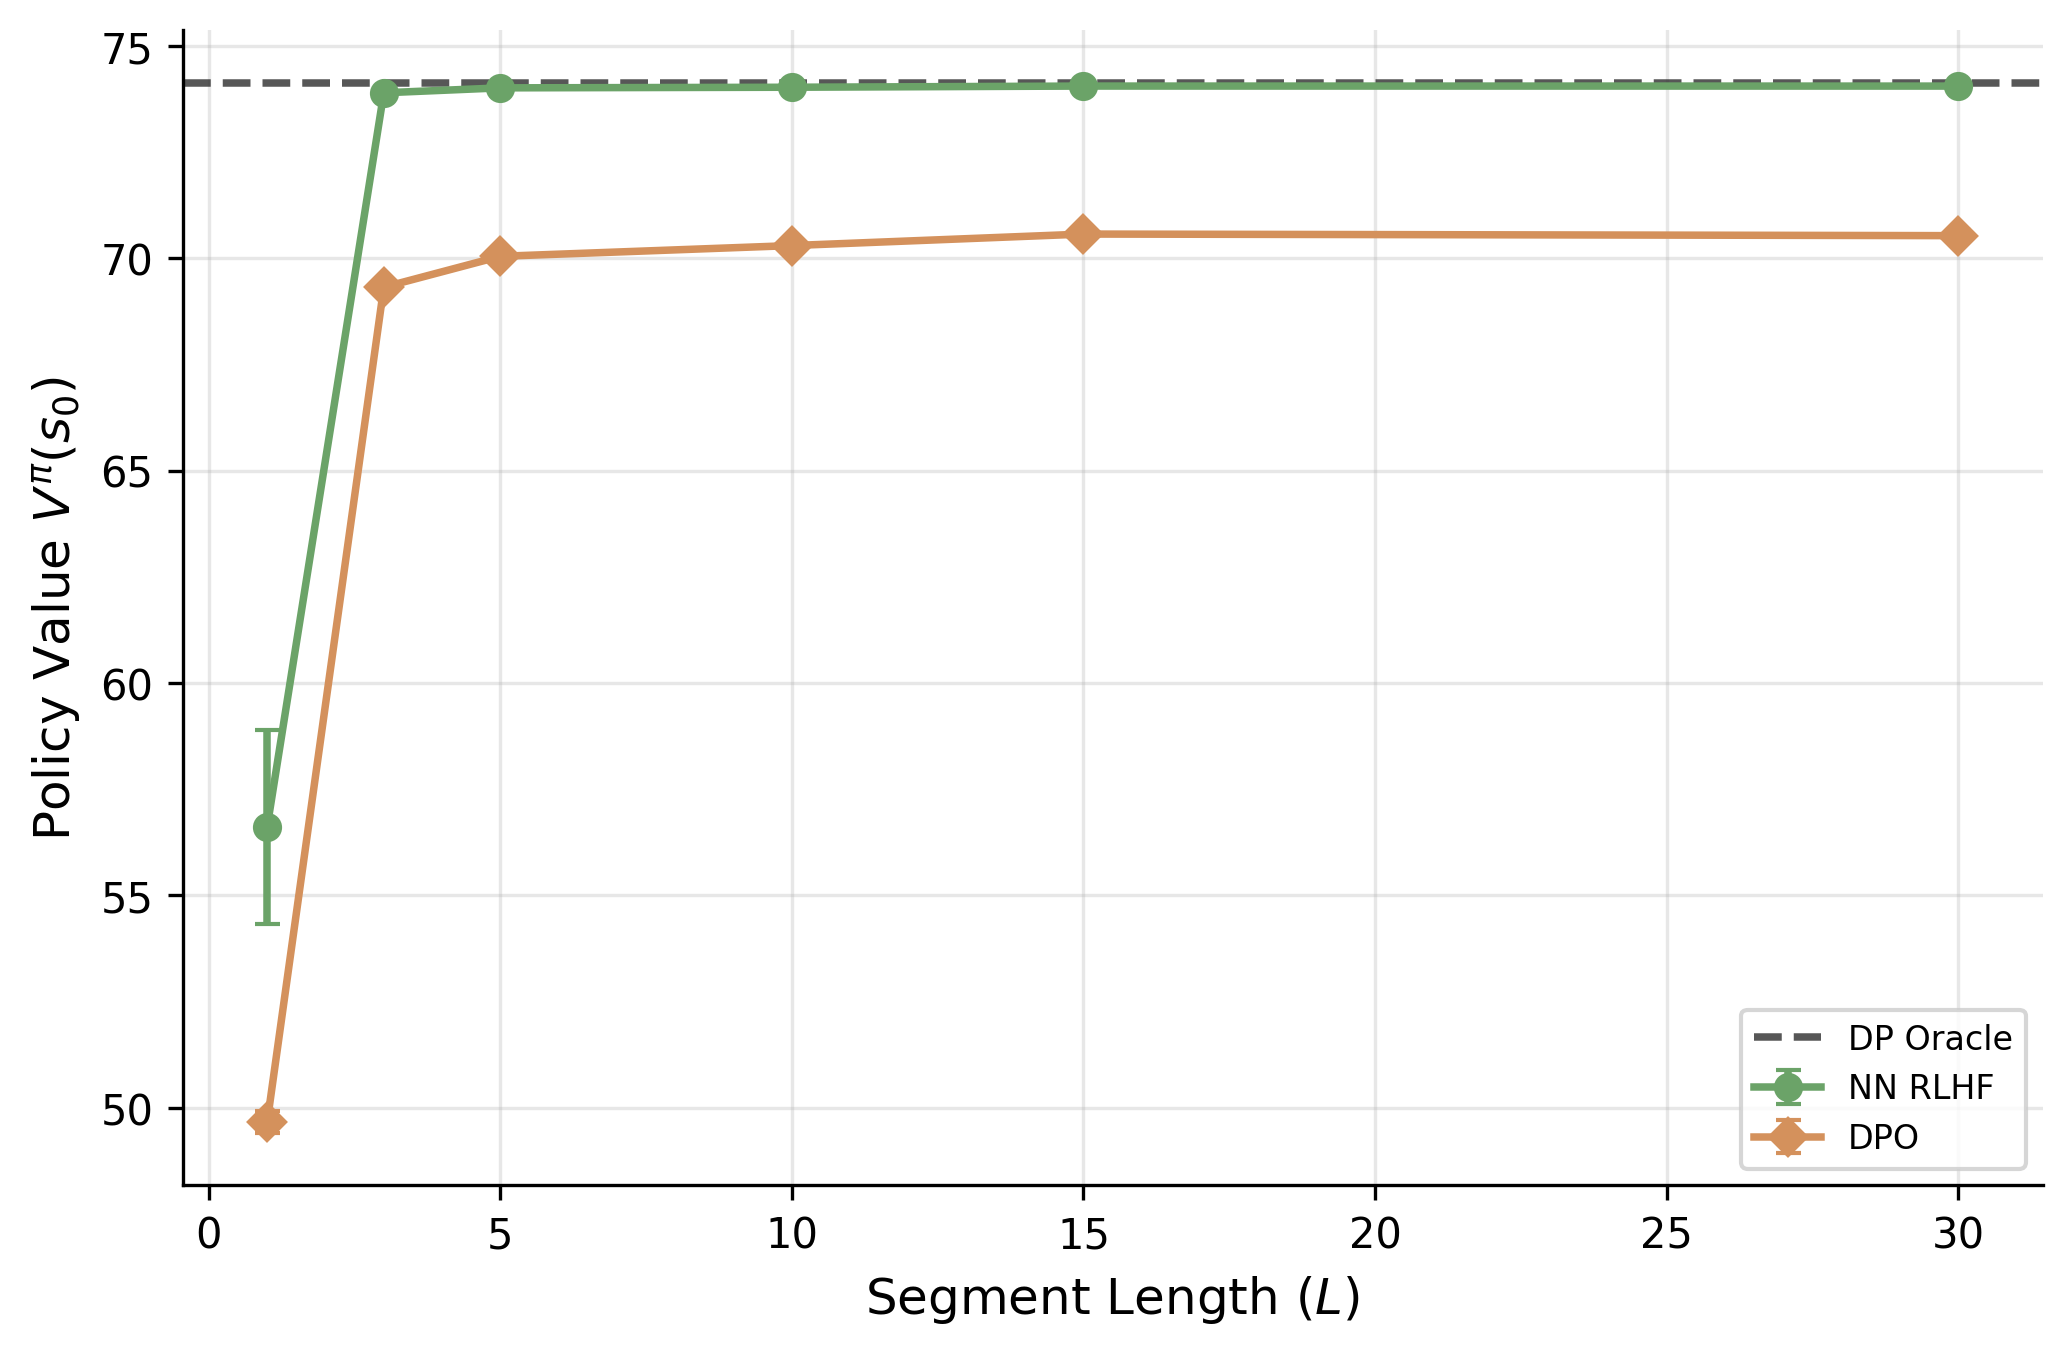
\includegraphics[width=0.7\textwidth]{../ch08_rlhf/sims/job_search_horizon.png}
\caption{Policy value $V^\pi(s_0)$ versus segment length $L$ at $K = 2{,}000$ for the neural network and DPO.}
\label{fig:preference_horizon}
\end{figure}

Table~\ref{tab:preference_horizon} and Figure~\ref{fig:preference_horizon} report the segment length ablation at $K = 2{,}000$. At $L = 1$, both methods perform poorly because single-step comparisons carry minimal information about long-run value. The neural network recovers rapidly (by $L = 3$) because the reward model aggregates per-transition estimates over longer segments and value iteration propagates them through the full transition structure; DPO improves monotonically but plateaus at its $\sim$95\% ceiling, as it must learn the policy directly from trajectory comparisons without access to the transition model.

Two-stage RLHF separates preference estimation (a static econometric problem) from dynamic programming (which exploits the known transition model); DPO conflates the two and forfeits the transition structure that economists typically have access to.\footnote{This advantage is specific to settings where the transition model is known or estimable; in domains without a tractable transition model, DPO's single-stage approach avoids compounding errors from reward model estimation.}

